\documentclass{article}
\usepackage[T1]{fontenc}
\usepackage{lmodern}
\usepackage{graphicx}
\usepackage{amsmath,amssymb}
\usepackage[a4paper,margin=2cm]{geometry}
\usepackage[absolute,overlay]{textpos}
\setlength{\TPHorizModule}{1mm}
\setlength{\TPVertModule}{1mm}
\usepackage[indonesian]{babel}
\usepackage{hyperref}
\setlength{\emergencystretch}{2em}
% unit: Halaman 110

\begin{document}

% === Halaman 110 (llm) ===

\vspace{136.62mm}

Sumber gambar: https://www.101computing.net/enigma/enigma-instructions.html
\vspace{10mm}
Operator mengetik huruf plainteks pada keyboard, lalu menyalin ulang huruf cipherteks yang menyala pada \textit{lampboard}. Cipherteks dikirim ke penerima pesan

% deskripsi: Ilustrasi simulasi mesin Enigma yang menunjukkan komponen Lampboard, Rotors, Keyboard, dan Plugboard beserta penjelasannya.
% bbox normalisasi: [0.1200, 0.2200, 0.8700, 0.6800]
\begin{textblock*}{157.50mm}(25.20mm,65.34mm)
\noindent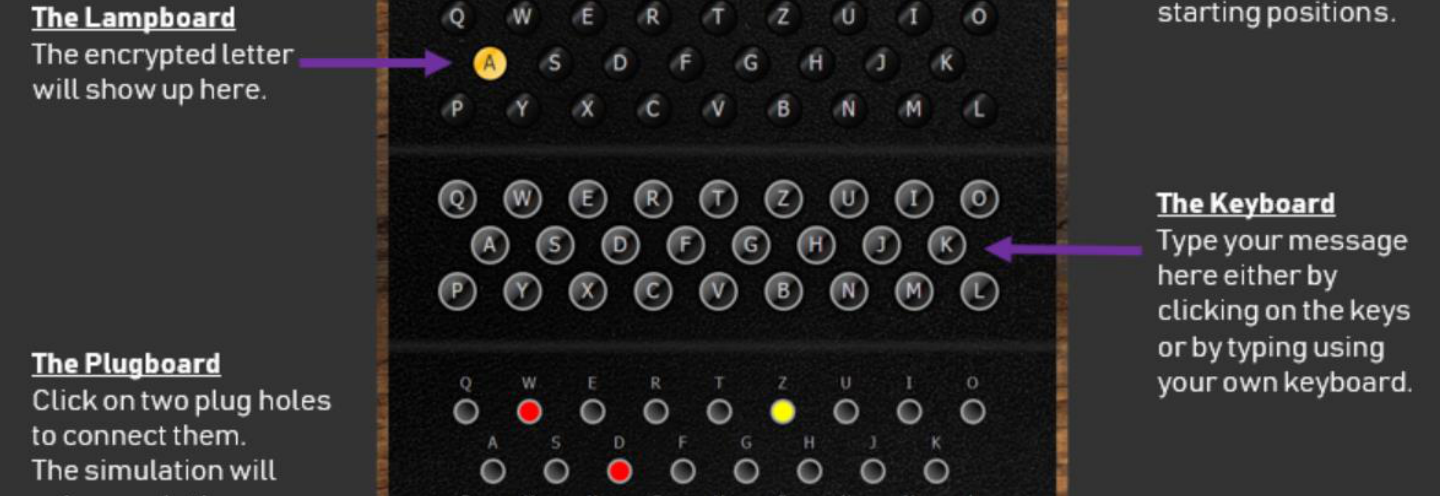
\includegraphics[width=157.50mm,height=136.62mm]{../../images/llm/page_110_img_01.png}%
\end{textblock*}

\end{document}
